\section{Additional results}
\label{app:results}


\begin{table*}[t]
\centering
\scriptsize
\setlength{\tabcolsep}{3.5pt}
\caption{Optimizer tokens in millions and wall clock per arm, summed over seeds. Non-cache-read tokens are uncached input, output and cache writes, the quantity the optimizer cap of 4M per search counts. The last token column adds cache reads, which the cap ignores. Cap used is the largest seed as a share of the cap. (placeholder)}
\label{tab:cost_tokens}
\begin{tabular}{lrrrrrr}
\toprule
Arm & Rollouts at $B^\ast$ & Non-cache-read & Cache read & Incl.\ cache read & Cap used (\%) & Wall clock (h) \\
\midrule
\multicolumn{7}{l}{\textit{Suite A, SpreadsheetBench verified-400 (Gemma-4-31B-it)}} \\
\midrule
Meta-Harness & \pend{395} & \pend{5.1} & \pend{63.9} & \pend{69.0} & \pend{51} & \pend{6.4} \\
EvoSkill & \pend{393} & \pend{3.4} & \pend{36.7} & \pend{40.1} & \pend{34} & \pend{14.3} \\
GEPA & \pend{397} & \pend{2.2} & \pend{4.1} & \pend{6.4} & \pend{22} & \pend{22.5} \\
Trace2Skill & \pend{388} & \pend{5.5} & \pend{6.6} & \pend{12.1} & \pend{55} & \pend{24.4} \\
MIPROv2 & \pend{399} & \pend{3.7} & \pend{0.8} & \pend{4.5} & \pend{37} & \pend{22.4} \\
ACE & \pend{396} & \pend{5.2} & \pend{5.4} & \pend{10.7} & \pend{52} & \pend{27.8} \\
WikiSkill (community) & \pend{393} & \pend{2.2} & \pend{3.4} & \pend{5.6} & \pend{22} & \pend{28.3} \\
SkillOpt & \pend{393} & \pend{3.9} & \pend{0.8} & \pend{4.7} & \pend{39} & \pend{19.6} \\
CapEvolve HC & \pend{394} & \pend{4.3} & \pend{78.6} & \pend{82.9} & \pend{43} & \pend{24.1} \\
CapEvolve AO & \pend{386} & \pend{7.2} & \pend{73.6} & \pend{80.8} & \pend{72} & \pend{16.7} \\
CapEvolve HC, stock gate \textit{(exploratory)} & \pend{396} & \pend{6.2} & \pend{96.4} & \pend{102.6} & \pend{62} & \pend{9.1} \\
\midrule
\multicolumn{7}{l}{\textit{Suite B, $\tau^2$ retail, sealed test-40 (gpt-oss-120b)}} \\
\midrule
One-shot control & \pend{10} & \pend{0.6} & \pend{2.1} & \pend{2.7} & \pend{6} & \pend{0.8} \\
GEPA & \pend{338} & \pend{3.0} & \pend{3.5} & \pend{6.5} & \pend{30} & \pend{18.1} \\
HarnessLens & \pend{336} & \pend{4.6} & \pend{6.7} & \pend{11.3} & \pend{46} & \pend{11.2} \\
CapEvolve HC & \pend{342} & \pend{7.9} & \pend{118.4} & \pend{126.3} & \pend{79} & \pend{15.6} \\
CapEvolve AO & \pend{350} & \pend{3.7} & \pend{109.7} & \pend{113.4} & \pend{37} & \pend{10.9} \\
\midrule
\multicolumn{7}{l}{\textit{Suite C, $\tau^2$ airline, official test-20 (development-exposed)}} \\
\midrule
One-shot control & \pend{10} & \pend{0.6} & \pend{6.8} & \pend{7.4} & \pend{6} & \pend{1.0} \\
HarnessLens & \pend{241} & \pend{1.9} & \pend{3.2} & \pend{5.1} & \pend{19} & \pend{7.4} \\
GEPA & \pend{245} & \pend{5.1} & \pend{3.5} & \pend{8.5} & \pend{51} & \pend{13.9} \\
CapEvolve HC & \pend{245} & \pend{4.1} & \pend{107.7} & \pend{111.8} & \pend{41} & \pend{20.1} \\
CapEvolve AO & \pend{247} & \pend{4.8} & \pend{119.0} & \pend{123.8} & \pend{48} & \pend{25.4} \\
CapEvolve HC, stock gate \textit{(exploratory)} & \pend{245} & \pend{7.6} & \pend{75.9} & \pend{83.5} & \pend{76} & \pend{29.8} \\
\bottomrule
\end{tabular}
\end{table*}

\begin{table*}[t]
\centering
\scriptsize
\setlength{\tabcolsep}{3.5pt}
\caption{Promotions per search for every arm, from the candidate logs, with the mean number of candidates evaluated. A promotion is a candidate that the arm's own acceptance rule put on its lineage. CapEvolve with rule P is a deliberately conservative configuration and is expected to promote rarely, and the stock-gate rows (E12) show the other side of that trade. (placeholder)}
\label{tab:promotions}
\begin{tabular}{lcccccr}
\toprule
Arm & Seed 0 & Seed 1 & Seed 2 & Mean per search & Candidates evaluated & Promoted (\%) \\
\midrule
\multicolumn{7}{l}{\textit{Suite A, SpreadsheetBench verified-400 (Gemma-4-31B-it)}} \\
\midrule
Meta-Harness & \pend{4} & \pend{1} & \pend{3} & \pend{2.7} & \pend{12.0} & \pend{22} \\
EvoSkill & \pend{4} & \pend{6} & \pend{1} & \pend{3.7} & \pend{11.3} & \pend{32} \\
GEPA & \pend{2} & \pend{6} & \pend{7} & \pend{5.0} & \pend{9.7} & \pend{52} \\
Trace2Skill & \pend{5} & \pend{5} & \pend{1} & \pend{3.7} & \pend{9.3} & \pend{39} \\
MIPROv2 & \pend{6} & \pend{5} & \pend{2} & \pend{4.3} & \pend{9.7} & \pend{45} \\
ACE & \pend{7} & \pend{4} & \pend{5} & \pend{5.3} & \pend{10.7} & \pend{50} \\
WikiSkill (community) & \pend{5} & \pend{7} & \pend{6} & \pend{6.0} & \pend{9.3} & \pend{64} \\
SkillOpt & \pend{3} & \pend{4} & \pend{6} & \pend{4.3} & \pend{9.0} & \pend{48} \\
CapEvolve HC & \pend{3} & \pend{3} & \pend{3} & \pend{3.0} & \pend{11.3} & \pend{26} \\
CapEvolve AO & \pend{2} & \pend{2} & \pend{2} & \pend{2.0} & \pend{11.7} & \pend{17} \\
CapEvolve HC, stock gate \textit{(exploratory)} & \pend{3} & \pend{2} & \pend{7} & \pend{4.0} & \pend{11.0} & \pend{36} \\
\midrule
\multicolumn{7}{l}{\textit{Suite B, $\tau^2$ retail, sealed test-40 (gpt-oss-120b)}} \\
\midrule
One-shot control & \pend{2} & \pend{2} & \pend{1} & \pend{1.7} & \pend{8.7} & \pend{19} \\
GEPA & \pend{3} & \pend{2} & \pend{3} & \pend{2.7} & \pend{10.0} & \pend{27} \\
HarnessLens & \pend{7} & \pend{4} & \pend{4} & \pend{5.0} & \pend{8.3} & \pend{60} \\
CapEvolve HC & \pend{2} & \pend{1} & \pend{0} & \pend{1.0} & \pend{7.7} & \pend{13} \\
CapEvolve AO & \pend{3} & \pend{1} & \pend{0} & \pend{1.3} & \pend{9.7} & \pend{14} \\
\midrule
\multicolumn{7}{l}{\textit{Suite C, $\tau^2$ airline, official test-20 (development-exposed)}} \\
\midrule
One-shot control & \pend{6} & \pend{4} & \pend{3} & \pend{4.3} & \pend{8.0} & \pend{54} \\
HarnessLens & \pend{2} & \pend{7} & \pend{7} & \pend{5.3} & \pend{9.7} & \pend{55} \\
GEPA & \pend{6} & \pend{4} & \pend{7} & \pend{5.7} & \pend{10.7} & \pend{53} \\
CapEvolve HC & \pend{1} & \pend{0} & \pend{0} & \pend{0.3} & \pend{8.0} & \pend{4} \\
CapEvolve AO & \pend{0} & \pend{1} & \pend{0} & \pend{0.3} & \pend{8.7} & \pend{4} \\
CapEvolve HC, stock gate \textit{(exploratory)} & \pend{5} & \pend{4} & \pend{7} & \pend{5.3} & \pend{7.7} & \pend{70} \\
\bottomrule
\end{tabular}
\end{table*}


\begin{figure*}[t]
\centering
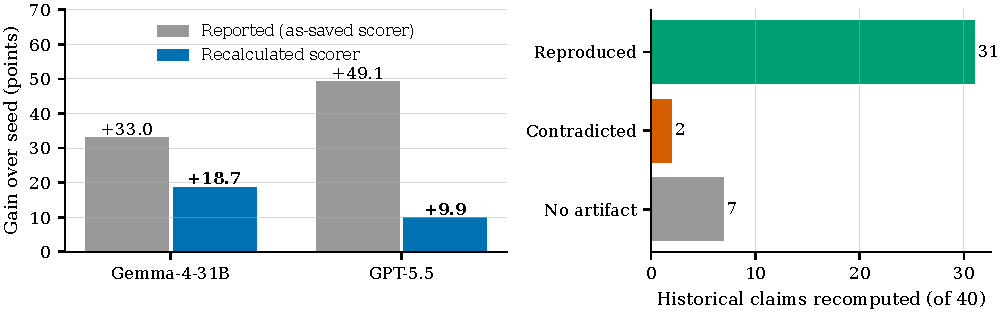
\includegraphics[width=\textwidth]{figures/fig_audit.pdf}
\caption{Recalculation removes most of the historical gain. Left: reported and recalculated gains of the two SpreadsheetBench headline runs. Right: outcome of recomputing every historical claim from archived artifacts (\texttt{audit/recomputed\_numbers.csv}).}
\label{fig:audit}
\end{figure*}

\begin{table*}[t]
\centering\scriptsize
\caption{Changes to each competitor's official code, from the per-arm deviation records (\texttt{baselines/deviations\_*.json}) and \texttt{decisions.md}. All arms share the same target rollout (Gemma-4-31B-it, 30 turns, gold-free sandbox), the same seed artifact, the same optimizer model (Claude Sonnet 5.5 through the gateway) and the same recalculated hard reward during search. ``Direction'' is our reading of how each change affects the arm relative to its published setting, not a measured effect.}
\label{tab:deviations}
\begin{tabularx}{\textwidth}{@{}l>{\raggedright\arraybackslash}X>{\raggedright\arraybackslash}X>{\raggedright\arraybackslash}p{1.9in}@{}}
\toprule
Arm & Change from the official code & Reason & Direction \\
\midrule
GEPA & Evaluator replaced by one CapEvolve rollout per example. Two text components (\texttt{prompt.md}, \texttt{task\_template.md}) updated round-robin. Every rollout counts against \texttt{max\_metric\_calls}. On Suite B the reflector is told to write only new guidance. & Same evaluator and artifact for all arms; rollout-matched budget. & Neutral for the search rule. Editing one component per proposal may slow progress on a two-file artifact. \\
SkillOpt & Rollout replaced. The two files are packed into one document. Native gold-to-agent training feedback and gold-versus-prediction reports removed. Test evaluation switched off. Optimizer temperature 0.7. & Gold-free comparison; test scored only by the campaign harness. & Lowers SkillOpt against its paper setting, because it loses oracle feedback. \\
Meta-Harness & Proposer \textsc{SKILL.md} written by us, since the upstream file is not public. Candidates are the two files, not a Python harness. Four iterations of two candidates, not about twenty. Final pick by validation mean, not Pareto frontier. Sonnet 5.5 at high effort, not Opus 4.6 at maximum. & Missing upstream file; same artifact; 600-rollout budget; matched optimizer model. & Lowers the arm: far fewer iterations and a weaker proposer. \\
EvoSkill & Base agent replaced by a CapEvolve rollout. Skills are appended to the system prompt, and skill scripts cannot run. Binary pass or fail from the recalculated score. Train pools by instruction type. Skill-only mode. & The CapEvolve agent loads only two files. & Probably lowers it, since progressive disclosure and skill tools are lost. Restarted once after the priority fault. \\
WikiSkill (community) & No official code exists, so we run the community port. Rollouts replaced. Role transport re-implemented as a tool loop on Sonnet 5.5, because the upstream transport is a Codex CLI. Skills appended to \texttt{prompt.md}. & Official code unavailable; matched optimizer model. & Unknown. The port may differ from the paper. \\
Trace2Skill & Repository's LLM-only error analyst, not the paper's agentic analyst with ground truth. README flags. A stand-in skill validator for a missing file. Uses about 200 of the 600 rollouts. & Gold-free protocol; repository omission; single-pass method. & Lowers it against the paper's strongest variant, which needs ground truth. Leaves budget unused. \\
ACE & Generator replaced by a counted CapEvolve rollout. No ground-truth mode. One reflection round, not three. Post-curator generation skipped. Output field \texttt{chain of thought} renamed to \texttt{analysis}. & Gold-free protocol; budget; the gateway returns an empty content-filter response for the original field. & Mildly lowers it (fewer rounds). The rename keeps the reflector's output usable. \\
MIPROv2 & One \texttt{dspy.Predict} whose instruction is the seed prompt. The forward pass builds \texttt{prompt.md} with demonstrations. Logging wrapper on candidate evaluation. About 400 rollouts natively. & The agent is multi-turn, not a single call; matched-checkpoint logging. & Neutral. Leaves part of the budget unused. \\
HarnessLens (Suite B) & Worker error retried once inside the budget; a second error scores zero for its internal selection only. Sandbox started with an environment allowlist. It is the only arm that streams the target. & Upstream aborts the whole stage on one worker error; isolation. & Unknown. A retry policy can lower its selection quality. \\
\bottomrule
\end{tabularx}
\end{table*}

\begin{table*}[t]
\centering
\scriptsize
\setlength{\tabcolsep}{3.5pt}
\caption{Paired delta to the seed for each search seed, in points, with the pessimistic and optimistic bounds on the mean. The pessimistic bound scores every missing cell of the arm as a loss and of the comparator as a win, and the optimistic bound does the reverse. Missing is missing over scheduled cells. (placeholder)}
\label{tab:perseed}
\begin{tabular}{lcccccr}
\toprule
Arm & Seed 0 & Seed 1 & Seed 2 & Mean $\Delta$ & Missingness bounds & Missing \\
\midrule
\multicolumn{7}{l}{\textit{Suite A, SpreadsheetBench, 70-task final set from the 912 residual pool (Gemma-4-31B-it)}} \\
\midrule
Meta-Harness & \pend{$-$2.9} & \pend{+0.4} & \pend{$-$0.9} & \pend{$-$1.1} & \pend{[$-$1.1, $-$1.1]} & \pend{0/210} \\
GEPA & \pend{+2.0} & \pend{+3.8} & \pend{+3.8} & \pend{+3.2} & \pend{[+0.8, +5.6]} & \pend{5/210} \\
EvoSkill & \pend{+4.7} & \pend{$-$0.1} & \pend{+6.1} & \pend{+3.6} & \pend{[+1.7, +5.5]} & \pend{4/210} \\
WikiSkill (community) & \pend{+5.4} & \pend{+5.0} & \pend{+5.4} & \pend{+5.3} & \pend{[+4.8, +5.8]} & \pend{1/210} \\
MIPROv2 & \pend{+5.0} & \pend{+6.1} & \pend{+4.8} & \pend{+5.3} & \pend{[+4.8, +5.8]} & \pend{1/210} \\
Trace2Skill & \pend{+4.1} & \pend{+6.0} & \pend{+6.4} & \pend{+5.5} & \pend{[+5.5, +5.5]} & \pend{0/210} \\
ACE & \pend{+4.7} & \pend{+6.8} & \pend{+5.2} & \pend{+5.6} & \pend{[+3.2, +8.0]} & \pend{5/210} \\
SkillOpt & \pend{+6.4} & \pend{+4.2} & \pend{+7.3} & \pend{+6.0} & \pend{[+5.5, +6.5]} & \pend{1/210} \\
CapEvolve as shipped, stock gate$^{\S}$ & \pend{+2.5} & \pend{+4.3} & \pend{+6.5} & \pend{+4.4} & \pend{[+0.6, +8.2]} & \pend{8/210} \\
CapEvolve HC, rule P & \pend{+1.5} & \pend{+5.9} & \pend{+2.2} & \pend{+3.2} & \pend{[+0.8, +5.6]} & \pend{5/210} \\
CapEvolve AO, rule P & \pend{+3.6} & \pend{+4.3} & \pend{+4.3} & \pend{+4.1} & \pend{[$-$0.2, +8.4]} & \pend{9/210} \\
\midrule
\multicolumn{7}{l}{\textit{Suite B, $\tau^2$ retail, sealed test-40 (gpt-oss-120b)}} \\
\midrule
One-shot control & \pend{+1.8} & \pend{+2.3} & \pend{+3.4} & \pend{+2.5} & \pend{[+2.2, +2.8]} & \pend{1/360} \\
GEPA & \pend{+1.0} & \pend{+4.1} & \pend{+2.9} & \pend{+2.7} & \pend{[+1.9, +3.5]} & \pend{3/360} \\
HarnessLens & \pend{+6.8} & \pend{+6.0} & \pend{+6.8} & \pend{+6.5} & \pend{[+6.5, +6.5]} & \pend{0/360} \\
CapEvolve HC, rule P & \pend{+4.1} & \pend{+0.0} & \pend{+4.0} & \pend{+2.7} & \pend{[+2.7, +2.7]} & \pend{0/360} \\
CapEvolve AO, rule P & \pend{+0.0} & \pend{+10.2} & \pend{+8.6} & \pend{+6.3} & \pend{[+4.9, +7.7]} & \pend{5/360} \\
\midrule
\multicolumn{7}{l}{\textit{Suite C, $\tau^2$ airline, official test-20 (development-exposed)}} \\
\midrule
One-shot control & \pend{+3.6} & \pend{+2.9} & \pend{+3.8} & \pend{+3.4} & \pend{[+2.3, +4.5]} & \pend{2/180} \\
GEPA & \pend{+1.8} & \pend{+0.2} & \pend{+0.7} & \pend{+0.9} & \pend{[$-$1.9, +3.7]} & \pend{5/180} \\
HarnessLens & \pend{+2.0} & \pend{+4.4} & \pend{+4.3} & \pend{+3.6} & \pend{[+3.6, +3.6]} & \pend{0/180} \\
CapEvolve as shipped, stock gate$^{\S}$ & \pend{+5.8} & \pend{+5.7} & \pend{+8.8} & \pend{+6.8} & \pend{[+6.2, +7.4]} & \pend{1/180} \\
CapEvolve HC, rule P & \pend{+6.4} & \pend{+3.4} & \pend{+3.5} & \pend{+4.4} & \pend{[+1.1, +7.7]} & \pend{6/180} \\
CapEvolve AO, rule P & \pend{+7.8} & \pend{+5.7} & \pend{+4.5} & \pend{+6.0} & \pend{[+6.0, +6.0]} & \pend{0/180} \\
One-shot best of $k$ & \pend{+0.3} & \pend{+0.7} & \pend{+0.5} & \pend{+0.5} & \pend{[$-$0.6, +1.6]} & \pend{2/180} \\
\bottomrule
\end{tabular}
\end{table*}


\begin{figure*}[t]
\centering
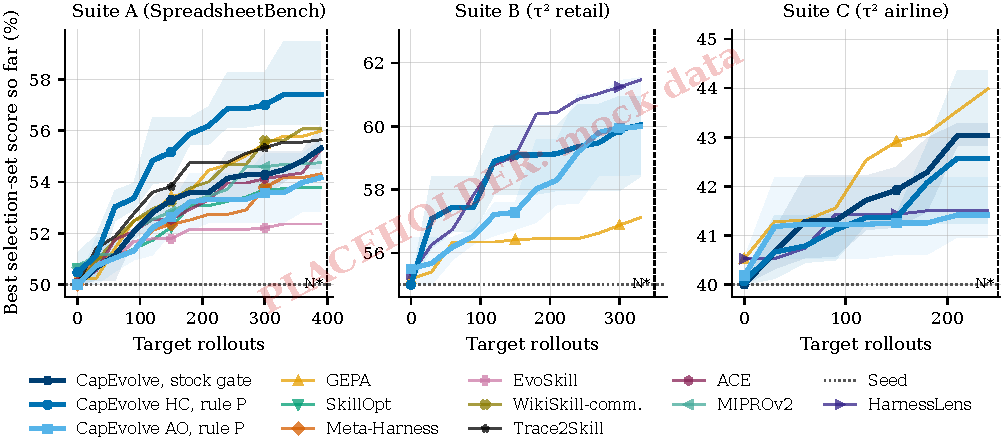
\includegraphics[width=\textwidth]{figures/fig_anytime.pdf}
\caption{Best selection-set score so far against target rollouts, with the matched checkpoint \ckpt{} dashed. The selection set is the 40 validation tasks on Suite A and the selection split on Suites B and C. Lines are averages over seeds, and bands are the minimum to maximum of the CapEvolve arms. The one-shot control has no curve because it makes one optimizer pass, and Suite A has no such control (placeholder).}
\label{fig:anytime}
\end{figure*}

\begin{figure*}[t]
\centering
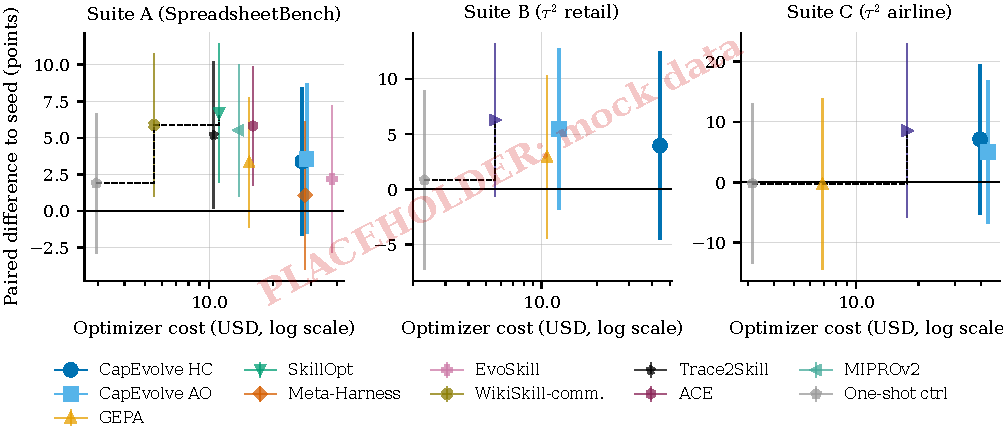
\includegraphics[width=\textwidth]{figures/fig_pareto.pdf}
\caption{Delta against optimizer cost, with the non-dominated arms joined by a dashed line. Cost is USD at Sonnet list prices on a log axis, and vertical bars are 95\% intervals (placeholder).}
\label{fig:pareto}
\end{figure*}

\begin{figure}[t]
\centering
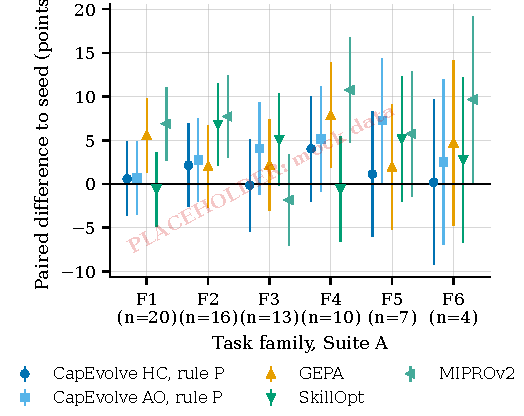
\includegraphics[width=\columnwidth]{figures/fig_families.pdf}
\caption{Delta by task family on Suite A for the main arms. Families are the cluster unit of the intervals (placeholder).}
\label{fig:families}
\end{figure}

\begin{figure*}[t]
\centering
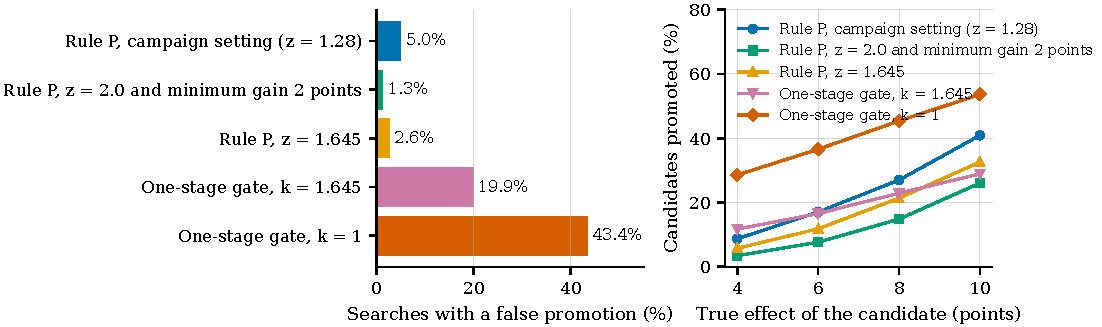
\includegraphics[width=\textwidth]{figures/fig_rulep.pdf}
\caption{Rule P promotes false candidates rarely and real ones less often than the one-stage gate. Left: share of all-null searches of six candidates with at least one false promotion. Right: share of single candidates promoted, against their true effect. The letter z is the confirmation threshold of rule P and k the threshold of the one-stage gate, both in standard errors. Source: \texttt{analysis/out/sim\_budget.md}.}
\label{fig:rulep}
\end{figure*}

\begin{figure*}[t]
\centering
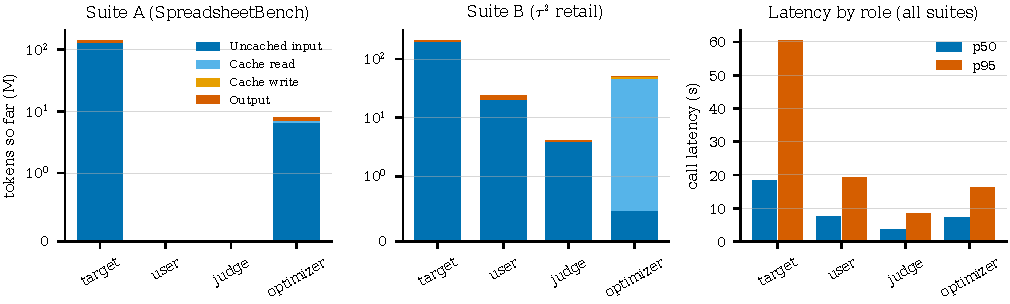
\includegraphics[width=\textwidth]{figures/fig_roles.pdf}
\caption{Target calls dominate tokens, and target calls are the slowest. Left and middle: tokens by kind for Suites A and B on a symmetric log axis. Right: call-weighted median and 95th-percentile latency per role. Main-category runs so far, in progress.}
\label{fig:roles}
\end{figure*}


\begin{table*}[t]
\centering
\scriptsize
\setlength{\tabcolsep}{3.5pt}
\caption{Campaign cost so far, from the gateway ledger (\texttt{analysis/out/metrics}). In progress: searches are still running, so every number is \prov{provisional}. Optimizer columns sum the optimizer, proposer, reflector and curator roles over seeds, in millions of tokens. The optimizer cap counts non-cache-read tokens, which are uncached input plus output plus cache writes, and applies to each search separately; the table shows the largest seed against the cap of 4M. Cache reads are listed apart and are not counted by the cap. ``0 (not started)'' means the arm is still in its baseline phase and has made no optimizer call yet; the optimizer is metered at the gateway once it runs, and the metering audit (\texttt{bypassed\_usage.csv}) found no optimizer usage outside the gateway. A double dagger would mark usage recovered from CLI transcripts. USD is a Sonnet list-price proxy for metered optimizer calls only and is a lower bound. Target tokens are uncached plus output tokens of the evaluated model. Wall is hours since launch for the longest seed. Errors count gateway calls that returned an error status, retries included. Rows count seeds that exist in the ledger.}
\label{tab:cost_so_far}
\begin{tabular}{llrrrrrrrrrr}
\toprule
Suite & Arm & Seeds & Rollouts & Opt.\ non-cache-read & Opt.\ cache read & Opt.\ incl.\ cache read & Cap used (\%) & Opt.\ USD & Target tok. (M) & Wall (h) & Errors \\
\midrule
A & CapEvolve HC & 3 & \prov{248} & \prov{0 (not started)} & \prov{0} & \prov{0} & \prov{0} & \prov{0} & \prov{14.79} & \prov{6.5} & \prov{0} \\
A & CapEvolve AO & 3 & \prov{223} & \prov{0 (not started)} & \prov{0} & \prov{0} & \prov{0} & \prov{0} & \prov{14.90} & \prov{6.4} & \prov{0} \\
A & GEPA & 3 & \prov{629} & \prov{0.34} & \prov{0.00} & \prov{0.34} & \prov{5} & \prov{1.15} & \prov{18.68} & \prov{12.8} & \prov{14} \\
A & SkillOpt & 3 & \prov{554} & \prov{2.83} & \prov{0.00} & \prov{2.83} & \prov{25} & \prov{6.59} & \prov{25.88} & \prov{12.8} & \prov{25} \\
A & Meta-Harness & 3 & \prov{589} & \prov{0.14} & \prov{0.55} & \prov{0.69} & \prov{1} & \prov{0.59} & \prov{28.82} & \prov{10.2} & \prov{15} \\
A & EvoSkill & 3 & \prov{117} & \prov{0 (not started)} & \prov{0} & \prov{0} & \prov{0} & \prov{0} & \prov{6.61} & \prov{2.7} & \prov{0} \\
A & WikiSkill & 3 & \prov{300} & \prov{0 (not started)} & \prov{0} & \prov{0} & \prov{0} & \prov{0} & \prov{17.62} & \prov{8.1} & \prov{0} \\
A & Trace2Skill & 3 & \prov{436} & \prov{6.51} & \prov{0.00} & \prov{6.51} & \prov{56} & \prov{20.27} & \prov{21.82} & \prov{12.3} & \prov{26} \\
A & ACE & 3 & \prov{74} & \prov{1.11} & \prov{0.00} & \prov{1.11} & \prov{12} & \prov{2.98} & \prov{7.90} & \prov{8.1} & \prov{0} \\
A & MIPROv2 & 3 & \prov{129} & \prov{0.54} & \prov{0.00} & \prov{0.54} & \prov{5} & \prov{1.77} & \prov{6.11} & \prov{8.1} & \prov{1} \\
\midrule
B & CapEvolve HC & 3 & \prov{441} & \prov{0.87} & \prov{9.96} & \prov{10.83} & \prov{11} & \prov{4.91} & \prov{60.75} & \prov{8.5} & \prov{58} \\
B & CapEvolve AO & 3 & \prov{369} & \prov{2.09} & \prov{30.97} & \prov{33.07} & \prov{19} & \prov{12.95} & \prov{46.78} & \prov{8.5} & \prov{54} \\
B & GEPA & 3 & \prov{483} & \prov{0.61} & \prov{0.00} & \prov{0.61} & \prov{5} & \prov{2.15} & \prov{38.53} & \prov{8.5} & \prov{42} \\
B & one-shot ctrl & 3 & \prov{394} & \prov{0.51} & \prov{6.90} & \prov{7.41} & \prov{5} & \prov{3.15} & \prov{36.02} & \prov{5.1} & \prov{21} \\
B & seed ctrl & 3 & \prov{294} & \prov{0 (no optimizer)} & \prov{0} & \prov{0} & \prov{0} & \prov{0} & \prov{33.13} & \prov{6.8} & \prov{27} \\
\midrule
C & CapEvolve HC & 3 & \prov{60} & \prov{0.32} & \prov{3.51} & \prov{3.83} & \prov{3} & \prov{1.81} & \prov{10.43} & \prov{2.8} & \prov{19} \\
C & CapEvolve AO & 3 & \prov{100} & \prov{0.66} & \prov{9.16} & \prov{9.82} & \prov{7} & \prov{3.97} & \prov{8.31} & \prov{2.8} & \prov{5} \\
C & GEPA & 3 & \prov{90} & \prov{0.08} & \prov{0.00} & \prov{0.08} & \prov{1} & \prov{0.30} & \prov{5.96} & \prov{2.8} & \prov{2} \\
C & one-shot ctrl & 3 & \prov{100} & \prov{0.33} & \prov{4.58} & \prov{4.90} & \prov{3} & \prov{2.13} & \prov{11.07} & \prov{2.8} & \prov{11} \\
C & seed ctrl & 3 & \prov{0} & \prov{0 (no optimizer)} & \prov{0} & \prov{0} & \prov{0} & \prov{0} & \prov{8.50} & \prov{2.8} & \prov{7} \\
\bottomrule
\end{tabular}
\end{table*}


\begin{table}[t]
\centering
\scriptsize
\caption{Selected historical claims and their recomputation from archived artifacts (40 claims in total).}
\label{tab:audit}
\begin{tabularx}{\columnwidth}{@{}p{0.9in}X@{}}
\toprule
Claim & Recomputation \\
\midrule
Gemma +33.0 [29.1, 36.8] & reproduces; interval is pooled over observations, task-clustered is [26.9, 39.2]; +18.7 under recalculation \\
GPT-5.5 +49.1 [45.5, 52.8] & reproduces; recalculated gain is +9.9 \\
GPT-5.5 recalculated baseline 77.5 & reproduces; 110 of 217 recalculated passes need formulas \\
no-capability control 62.9 & same run's one-iteration hill climb scores 85.6, absent from the draft \\
run excluded for different commit & 55 of 280 rollouts hit a budget error; baseline 28.9 is on 225 tasks \\
SkillsBench 55.6 to 66.7 held out & the whole delta is one trial of one task \\
SWE-bench pilot 68.0, candidate 72.0 & candidate rejected; the seed scores 63.6 and 70.5 on the same 44 tasks \\
$\tau^2$ retail 0.460 to 0.545 & arithmetic only; no per-task artifact exists \\
$\tau^2$ held-out 30.0 to 47.5 & artifact never landed; runner identity differs between docs \\
\bottomrule
\end{tabularx}
\end{table}

